\section{Introduction to Boosting}
%
\begin{frame}
  Boosting encompasses an entire family highly successful learning algorithms.
\end{frame}
%
\begin{frame}
Boosting can adapt itself effortlessly to very non-linear objectives
  \only<1>{
    \begin{figure}
      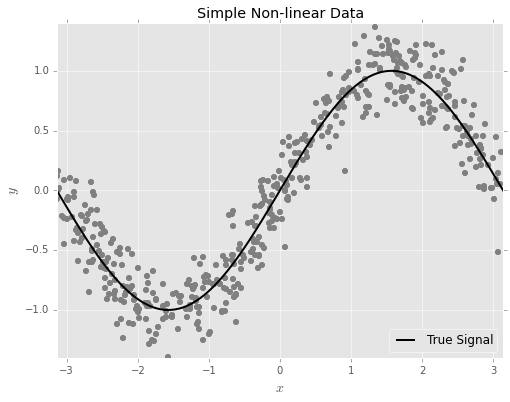
\includegraphics[scale=0.50]{sin-with-data}
    \end{figure}
   }
   \only<2>{
    \begin{figure}
      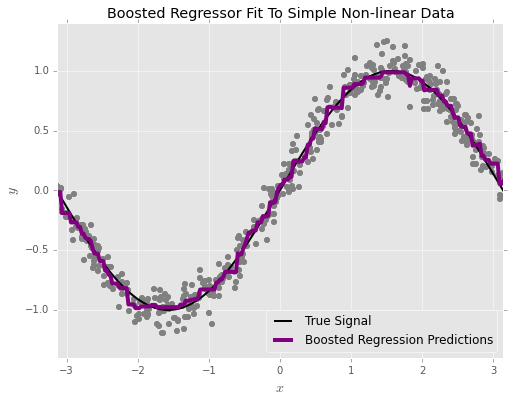
\includegraphics[scale=0.50]{sin-with-data-and-booster}
    \end{figure}
   }
   \only<3>{
    \begin{figure}
      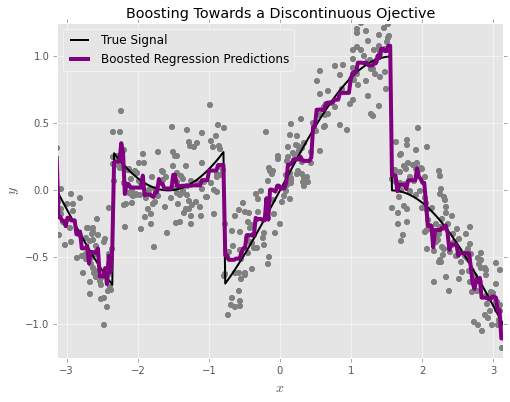
\includegraphics[scale=0.50]{broken-sin-with-booster}
    \end{figure}
   }
\end{frame}
%
\begin{frame}
Boosting accomplishes this by \textit{growing the model gradually}
  \begin{figure}
    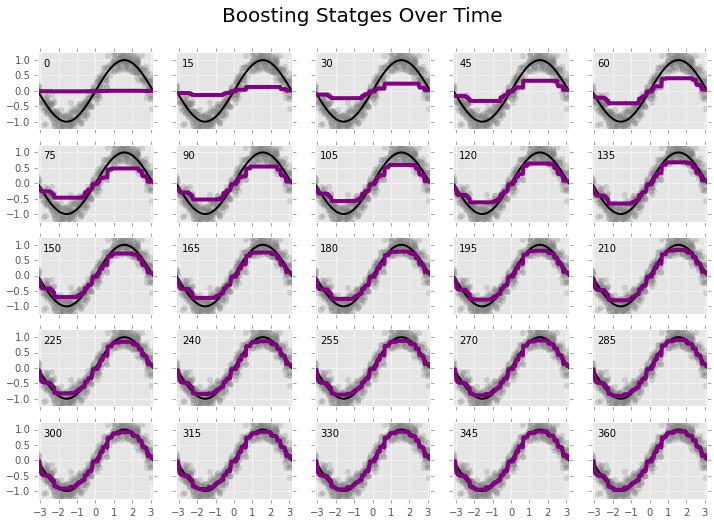
\includegraphics[scale=0.40]{boosting-over-time-multiple-plots}
  \end{figure}
\end{frame}
%
\begin{frame}
At each stage of the growth, the next model is built as an adjustment to the previous model
  \begin{figure}
    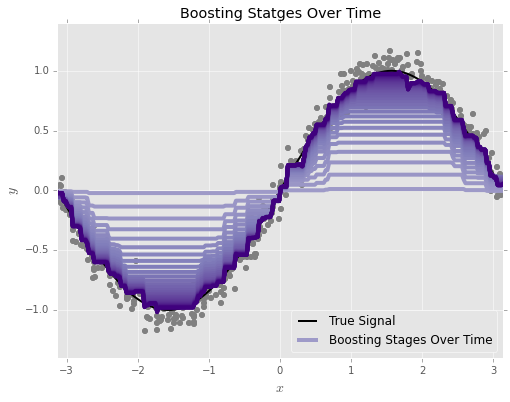
\includegraphics[scale=0.50]{boosting-over-time-single-plot}
  \end{figure}
\end{frame}
%
\begin{frame}

\only<2->{  
\textbf{Compared to}:\\~\\
}

\only<1>{
\textbf{Boosting}: \\~\\
Lowers variance by growing the model slowly over time (along with a few other tricks).\\~\\

Lowers bias by stacking many non-parametric models into the final result.
}

\only<2>{
\textbf{Linear Models}: \\~\\
Lowers variance by using a regularization penalty.\\~\\

Lowers bias by including more predictors.
}

\only<3>{
\textbf{SVM}: \\~\\
Lowers variance by maximizing the margin between positive and negative cases.\\~\\ 

Lowers bias by using a kernel, which projects the data into a very high dimensional space.
}

\only<4>{
\textbf{Random Forest}: \\~\\

Lowers variance by growing many learners on different subsamples of the data and predictors, then averaging them.\\~\\

Lowers bias by growing really big trees.
}

\end{frame}